\chapter{Návrh řešení}
\label{chap:navrh}

V této kapitole je představen detailní technický návrh prototypu CLI klienta a navazující síťové služby. Návrh přímo vychází ze zvolené architektury tenkého klienta, která byla zdůvodněna v předchozí kapitole (viz sekce \ref{sec:analyza_architektury}).

\section{Komponenty systému}
Celý systém je v souladu se zvoleným návrhem rozdělen na dvě hlavní, technologicky odlišné komponenty, které spolu komunikují přes definované rozhraní.

\begin{itemize}
    \item \textbf{Služba (Service - .NET):} Funguje jako daemon spravovaný systémem \texttt{systemd} s právy uživatele \texttt{root}. Její primární a jedinou odpovědností je správa stavu sítě, konfigurace rozhraní WireGuard a bezpečné ukládání kryptografických klíčů. Volba platformy .NET pro tuto komponentu přímo vychází z potřeby multiplatformní podpory a snadné integrace do systému \texttt{systemd} (viz sekce \ref{sec:technologie}), a především umožňuje znovupoužití již existující a otestované logiky z grafického klienta (viz sekce \ref{sec:analyza_architektury}).
    \item \textbf{Klient (Client - Go):} Běží v uživatelském prostoru (bez \texttt{root} oprávnění) a zajišťuje čistě interakci s uživatelem. Zodpovídá za parsování argumentů příkazové řádky pomocí frameworku \texttt{Cobra}, obsluhu interaktivních TUI prvků prostřednictvím \texttt{Bubble Tea} a finální formátování výstupu. Jazyk Go byl pro vývoj CLI zvolen díky svým vlastnostem pro systémové programování, rychlému startu a statické kompilaci do jediné binárky, což radikálně zjednodušuje distribuci (viz sekce \ref{sec:technologie} a \ref{sec:cli_teorie}).
\end{itemize}

Architektura Go klienta navíc úzce reflektuje principy takzvané \textit{Clean Architecture}. Celá kódová základna klienta je rozdělena do logických vrstev, kde uživatelské rozhraní (UI a parsování příkazů) je zcela odděleno od aplikační logiky a transportní vrstvy (IPC komunikace přes Unix Domain Sockets). Toto vrstvení zaručuje vysokou testovatelnost komponent a možnost nezávisle upravovat vizuální prezentaci bez vlivu na způsob, jakým klient komunikuje s .NET službou.

\begin{figure}[H]
    \centering
    % TODO: Přidat skutečný obrázek architektury
    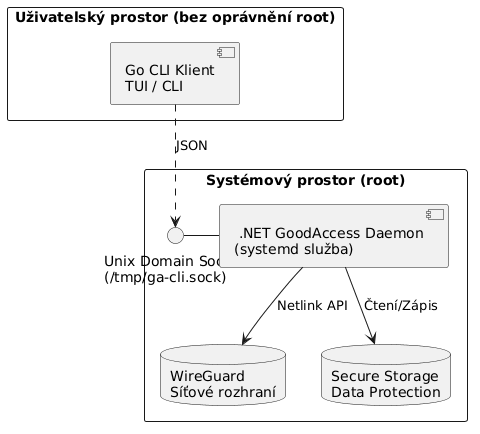
\includegraphics[width=0.8\textwidth]{images/navrh-architecture.png}
    \caption{Architektura systému znázorňující hranici mezi .NET Službou a Go Klientem skrze IPC (Unix Domain Sockets).}
    \label{fig:architecture_ipc}
\end{figure}

\begin{figure}[H]
    \centering
    % TODO: Přidat skutečný obrázek Clean Architecture
    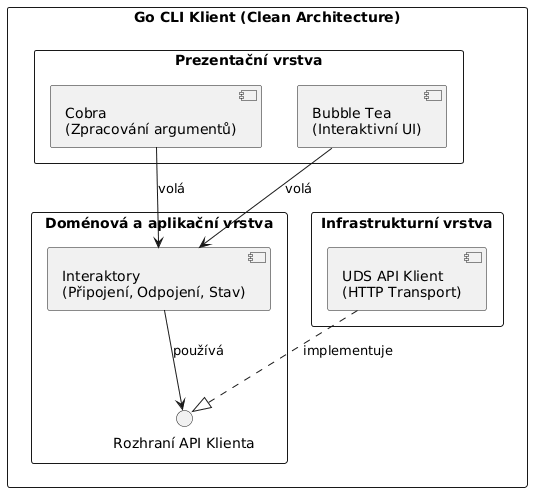
\includegraphics[width=0.8\textwidth]{images/clean-architecture.png}
    \caption{Struktura vrstev Go klienta v souladu s principy Clean Architecture.}
    \label{fig:clean_architecture_go}
\end{figure}

\section{Návrh komunikace IPC}
Pro výměnu dat mezi Go klientem a .NET službou bylo nutné zvolit vhodný mechanismus meziprocesní komunikace (IPC). Jak bylo popsáno v teoretické části (viz sekce \ref{sec:ipc_theory}), pro lokální komunikaci v systému Linux jsou nejvhodnějším nástrojem Unix Domain Sockets (UDS). Ty nabízejí vyšší bezpečnost díky souborovým oprávněním a lepší výkon oproti síťovým socketům (TCP/IP), protože nedochází k režii spojené se síťovým stackem.

\subsection{Volba formátu dat}
V teoretické kapitole (viz sekce \ref{sec:formats_theory}) byly porovnány formáty JSON a gRPC. Pro účely této práce byl zvolen formát \textbf{JSON}. Hlavním důvodem je jeho textová čitelnost, která výrazně usnadňuje ladění komunikace během vývoje, a nativní podpora v obou použitých jazycích (Go i C\#) bez nutnosti generovat složité stuby, což odpovídá agilnímu principu jednoduchosti.

\subsection{Protokol a struktura zpráv}
Komunikace probíhá podle modelu Request-Response. Klient otevře spojení k socketu služby (typicky \texttt{/var/run/goodaccess.sock}), odešle požadavek v JSON formátu a čeká na odpověď, po které spojení uzavře.

Průběh typické komunikace pro přihlášení uživatele znázorňuje následující sekvenční diagram (Obrázek \ref{fig:ipcsequence}).

\begin{figure}[H]
    \centering
    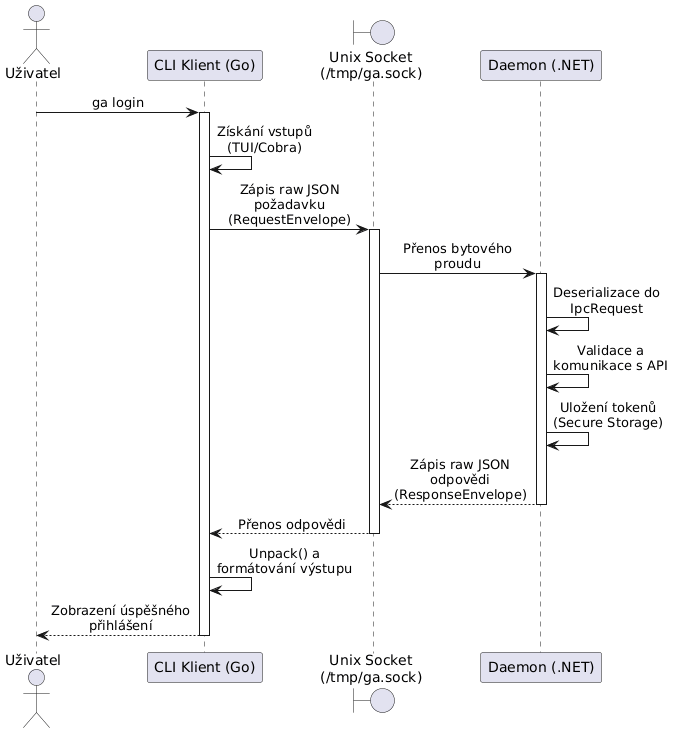
\includegraphics[width=0.8\textwidth]{images/ipc-sequence.png}
    \caption{Sekvenční diagram IPC komunikace při přihlášení.}
    \label{fig:ipcsequence}
\end{figure}

\subsection{Příklady zpráv}
Struktura požadavku obsahuje název příkazu (\texttt{command}), samotná data (\texttt{payload}) a kontext požadavku (\texttt{context}), který nese informace o volajícím uživateli.

Příklad požadavku na přihlášení (\texttt{login}):

\begin{minipage}{\linewidth}
\begin{lstlisting}[language={}]
{
  "command": "login",
  "payload": {
    "TeamName": "mojefirma",
    "UserName": "jan.novak@mojefirma.cz",
    "Password": "moje_tajne_heslo"
  },
  "context": {
    "LinuxId": "1000",
    "IsRoot": false
  }
}
\end{lstlisting}
\end{minipage}

Služba na tento požadavek odpovídá strukturovanou zprávou, která indikuje úspěch či selhání a vrací příslušná data nebo chybové hlášení.

Příklad úspěšné odpovědi:

\begin{minipage}{\linewidth}
\begin{lstlisting}[language={}]
{
  "success": true,
  "data": {
    "IsLoggedIn": true
  }
}
\end{lstlisting}
\end{minipage}

Příklad odpovědi při chybě (neplatné údaje):

\begin{minipage}{\linewidth}
\begin{lstlisting}[language={}]
{
  "success": false,
  "data": null,
  "error": "Invalid credentials"
}
\end{lstlisting}
\end{minipage}

\section{Návrh uživatelského rozhraní (CLI)}
% Zde:
% - Strom příkazů (ga login, ga connect, ga status).
% - Návrh interaktivního režimu (TUI) vs. skriptovacího režimu (flags).
% - Jak budou vypadat výstupy (barvičky pro lidi, JSON pro stroje).

\section{Bezpečnostní model}
% Zde:
% - Ukládání tokenů (kde budou fyzicky na disku).
% - Oprávnění k socketu (kdo smí poslat příkaz službě).
% - Zabezpečení proti neoprávněné manipulaci.

\section{Datový model a konfigurace}
% Zde:
% - Kde bude konfigurace (/etc/goodaccess vs ~/.config/goodaccess).
% - Co všechno se musí ukládat (aliasy bran, poslední připojení).
